\pdfoptionpdfminorversion=5
% \documentclass[9pt,hyperref={pdfpagelabels=false}]{beamer}
\documentclass[9pt]{beamer}

\mode<presentation> {
    \usetheme{HHUD}
    \setbeamercovered{invisible}
}
\usepackage[ngerman]{babel}
\usepackage[utf8x]{inputenc}
\usepackage{times}
\usepackage{amsmath}
\usepackage{subfigure}
\usepackage{graphicx}
\usepackage{hyperref}
\usepackage{xmpmulti}
\usepackage{multicol}
\usepackage{color}
\usepackage{appendixnumberbeamer}


% background image
\usebackgroundtemplate{
\includegraphics[width=\paperwidth]{fig/background}}
% commands for low and high decoration in frame foot
\newcommand{\footdecorationlow}{\usebackgroundtemplate{
\includegraphics[width=\paperwidth]{fig/background_small}}}
\newcommand{\footdecorationhigh}{\usebackgroundtemplate{
\includegraphics[width=\paperwidth]{fig/background}}}

 \AtBeginSection[] {
   \footdecorationhigh
   \begin{frame}<beamer>
     \thispagestyle{empty}
          \frametitle{Übersicht}
    \vspace{-5mm}
     \tableofcontents[currentsection]
   \end{frame}
   \footdecorationlow
 }

% % % % % % % % % %  CHANGE TOPIC AND AUTHOR INFORMATION HERE % % % % % % % % %
% \newcommand{\abschluss}{Master}                                             % HIER UNZUTREFFENDES LÖSCHEN
% \title{\abschluss{}arbeit:\\VANET-Protokolle f{\"u}r Kolonnenfahrten}           % HIER DEN TITEL DER ARBEIT EINTRAGEN
\title{Lokalisierung von Objekten in Bildern mittels neuronaler Netze}                                           % HIER DEN TITEL DER ARBEIT EINTRAGEN
\author{Projektarbeit \newline Deniz Ates}                                                    % HIER DEN NAMEN UND VORNAMEN EINTRAGEN
 \date{\today}                                                                % HIER DAS PRÄSENTATIONSDATUM EINTRAGEN
% % % % % % % % % % % % % % % % % % % % % % % % % % % % % % % % % % % % % % % %
\institute{Institut für Informatik\\Heinrich-Heine-Universität Düsseldorf}
\subject{Informatik}

% % % % % % % % % % Own commands % % % % % % % %

%
% Hier beginnt das Dokument
%
\begin{document}
	
	\footdecorationhigh
	\begin{frame}
	\thispagestyle{empty}
	\titlepage
\end{frame}

% Inhaltsverzeichnis - fuer kurze Vorträge eher weglassen
\begin{frame}
\thispagestyle{empty}
\frametitle{Übersicht}
\vspace{-5mm}
\tableofcontents
\end{frame}


% Fußzeile wieder niedrig setzen für normale Folien
\footdecorationlow

\section{Ziel der Projektabeit}  
\begin{frame}
\vspace{10pt}
\begin{block}{Ziel der Projektarbeit war es:}
	\begin{itemize}
		\item ...Fliesen und Fenster innerhalb eines Bildes automatisch zu erkennen.
		\item ...die Bereiche in denen sich Fliesen und Fenster befinden aus dem Originalbild zu extrahieren.
		\item ...auf Basis dieser Extraktion Schäden zu erkennen und in zukünftigen Schritten zu analysieren. 
	\end{itemize}
\end{block}
\end{frame}

\section{Datensatz}  
\begin{frame}
\begin{block}{Initialer Datensatz}
	\begin{itemize}
		\item Der gegebene Datensatz besteht aus aus jeweils 200 Schadensfällen pro Objektklasse (Fliese, Fenster, Dach usw.)
		\item Ein Schadensfall beinhaltet zwischen Einem und Acht Bildern.
		\item \textbf{Hauptproblem:} Die Bilder innerhalb der Klassen sind oftmals falsch Klassifiziert oder von sehr schlechter Qualität
		\item Somit konnte nur ein Bruchteil (knapp 50 Bilder aus dem original Datensatz) genutzt werden
		\item Um trotzdem einen representativen Datensatz zu erhalten, wurden Bilder aus ImageNet hinzugezogen, welche den verwendbaren Originalbildern in Struktur und Qualität ähnlich waren 
	\end{itemize}
\end{block}
\end{frame}


\begin{frame}{Auszug aus dem Datensatz}

\end{frame}

\section{Ansatz über Bildverarbeitung}  
\begin{frame}{Ziele der Bildverarbeitung}
\begin{block}{Direkte Extraktion der Objekte}
	\begin{itemize}
		\item Template Match
	\end{itemize}
\end{block}

\begin{block}{Automatische Generierung von Masken}
	\begin{itemize}
		\item GrabCut
		\item Backgroundextraction
		\item Contour Detection
	\end{itemize}
\end{block}

\begin{block}{Bildverarbeitung als Preprocessing für das neuronale Netz}
	\begin{itemize}
		\item Canny Edge 
		\item Filterung
	\end{itemize}
\end{block}
	
\end{frame}

\section{Pipeline}  	
\begin{frame}{Pipeline}
\begin{figure}
	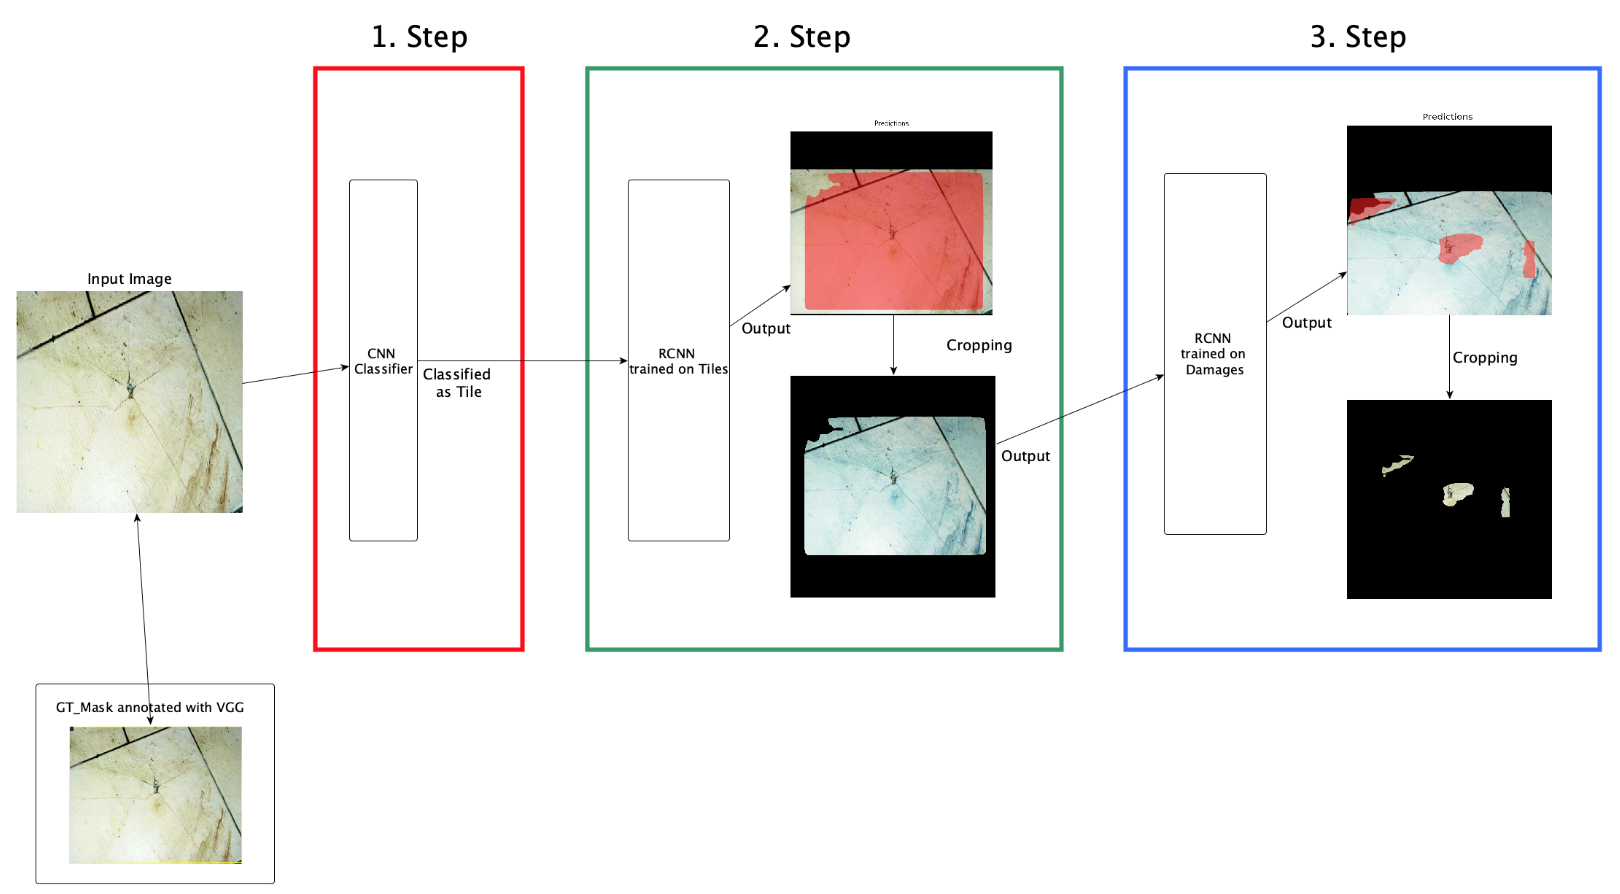
\includegraphics[width=\textwidth]{./fig/Pipeline.png}
	\caption{Illustration der Gesamtpipeline}
\end{figure}

\end{frame}
\subsection{1 - Klassifikation}
\begin{frame}{1 - Klassifikation}
\begin{figure}
	
\includegraphics[height=200px]{./fig/1}
	\caption{Erster Pipelineschritt}
\end{figure}
\end{frame}

\begin{frame}{1 - Klassifikation}
\begin{block}{Klassifikation mithilfe eines CNNs}
	\begin{itemize}
		\item CNN Architektur
		\item Daten: 110 Bilder mit Fliesen und 68 Bilder mit Fenstern
		\item 100 Epochen Trainingszeit
		\item 83\% richtig klassifizierte Bilder in einer Testmenge von 130 Bildern.
		
	\end{itemize}
\end{block}
\end{frame}

\subsection{2 - Erkennung einzelner Strukturen \& Objekte}
\begin{frame}{2 - Erkennung einzelner Strukturen \& Objekte}
\begin{figure}
	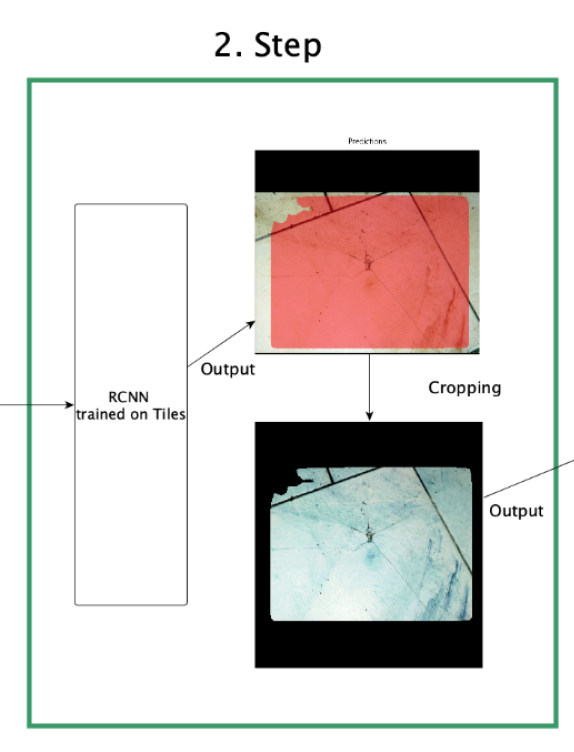
\includegraphics[height=200px]{./fig/2}
	\caption{Zweiter Pipelineschritt}
\end{figure}
\end{frame}

\begin{frame}
\begin{block}{Extraktion von Fliesen und Fenstern}
	\begin{itemize}
		\item RCNN Architektur
		\item RCNN Erklären
		\item Daten: 
		\item 100 Epochen Trainingszeit
		\item Evalergebnisse
		
	\end{itemize}
\end{block}
\end{frame}

\subsection{3 - Erkennung von Schäden innerhalb der Objekte}
\begin{frame}{3 - Erkennung von Schäden innerhalb der Objekte}
\begin{figure}
	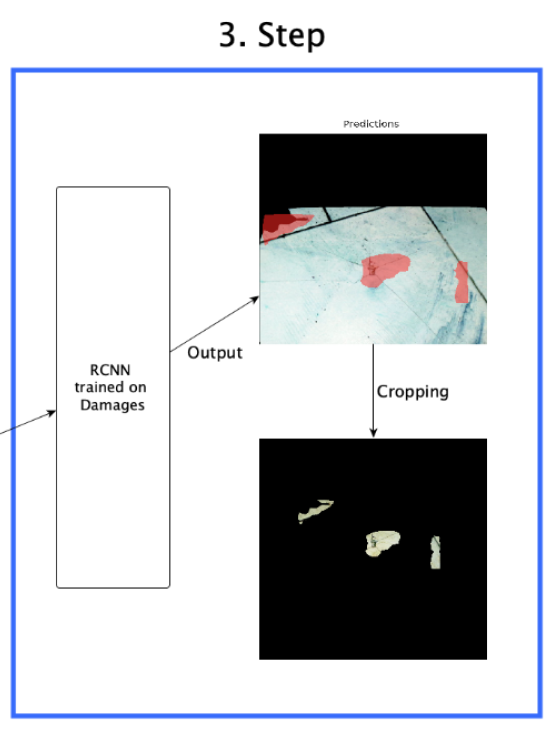
\includegraphics[height=200px]{./fig/3}
	\caption{Dritter Pipelineschritt}
\end{figure}
\end{frame}

\begin{frame}
\begin{block}{Extraktion von Schäden innerhalb der Masken}
\begin{itemize}
	\item RCNN Architektur
	\item RCNN Erklären
	\item Daten: 
	\item 100 Epochen Trainingszeit
	\item Evalergebnisse
	
\end{itemize}
\end{block}
\end{frame}
\section{Evaluation}  

\begin{frame}{Evaluationsergebnisse}

\end{frame}

\section{Future Work}  
\begin{frame}
Auf Basis der gewonnen Erkenntnisse ergeben sich folgende (mögliche) weiterführende Arbeiten:
\begin{block}{Allgemeine Verbesserung des Netzes}
	\begin{itemize}
		\item Vergrößerung der Datenmenge vorallem Schadensbilder (künstliche generierung von Schaden verbessern)
		\item Mehr Trainingsepochen und Anpassungen weitere Hyperparameter
		\item Pre \& Postprocessing vertiefen
	\end{itemize}
\end{block}
\begin{block}{4. Pipelineschritt}
	\begin{itemize}
		\item Klassifikation von Schäden (z.B Riss, Bruch, tiefe Schäden) 
		\item Metriken auf Schäden anwenden (wie z.B die größe des Schadens in Relation zur Maske)
	\end{itemize}
\end{block}
\end{frame}

\begin{frame}
\begin{block}{5. Pipelineschritt}
	\begin{itemize}
		\item Die Klassifizierten Schäden können nun mithilfe der textuellen Beschreibung eines Schadensfalles abgeglichen werden  
		\item Durch NLP können die Informationen der Textbeschreibung extrahiert werden und eine Prediction für den Kostenfaktor eines Schadens aufgestellt werden
	\end{itemize}
\end{block}
\textbf{Die gesamte Pipeline könnte somit automatisch die Plausibilität eines Schadensfalls und des Kostenvoranschlags ermitteln und Unregelmäßigkeiten sowie Ausreißer erkennen}
\end{frame}

\section{Referenzen} 
	\vspace*{0.5cm}
\begin{thebibliography}{10}
	\bibitem{paper1}Ian J. Goodfellow, Jonathon Shlens \& Christian Szegedy -\newline EXPLAINING AND HARNESSING
	ADVERSARIAL EXAMPLES - Google Inc., Mountain View, CA - 2015
	\bibitem{paper2}N. Papernot, P. McDaniel, I. Goodfellow, S. Jha, B. Celik, A. Swami
	 - Practical Black-Box Attacks against Machine Learning - 2017
	 \bibitem{paper3} Alexey Kurakin, Ian Goodfellow, Samy Bengio- \newline
	 Adversarial examples in the physical world - 2016
	  \bibitem{paper4}Papernot, Nicolas and Goodfellow, Ian and Sheatsley, Ryan and Feinman, Reuben and McDaniel, Patrick- \newline
  	 Cleverhans v1.0.0: an adversarial machine learning library- \newline
  	 \textbf{https://github.com/tensorflow/cleverhans}
	  \bibitem{paper5} Ian J. Goodfellow - Presentation of EXPLAINING AND HARNESSING
	  ADVERSARIAL EXAMPLES - \newline
	  Lecture 16 | Adversarial Examples and Adversarial Training \newline
	  \textbf{https://www.youtube.com/watch?v=CIfsBEYsVI}
\end{thebibliography}
\begin{frame}
\Huge \centering \textbf{Vielen Dank für Eure Aufmerksamkeit!}
\end{frame}

\end{document}

%
% Hier endet das Dokument
%